\clearpage\begingroup\SourceLeaf{105b}\HistoricalHead{100}{L}{PHYSIK. BRIEFWECHSEL.}
\newcommand{\HistoricalCurrencyLSeventeen}{%
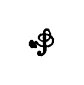
\begin{tikzpicture}[x=.075pt,y=-.075pt,baseline=-7.5pt]
\path[use as bounding box] (0,0) rectangle (134,141);
\path[fill=black,even odd rule]
(86,3) -- (86,4) -- (85,5) -- (84,5) -- (84,6) -- (83,7) -- (81,7) -- (81,9) -- (80,10) -- (79,10) -- (79,11) -- (78,12) -- (77,12) -- (77,15) -- (76,16) -- (75,16) -- (75,24) -- (74,25) -- (73,25) -- (73,26) -- (72,27) -- (71,27) -- (71,28) -- (70,29) -- (60,29) -- (60,30) -- (59,31) -- (58,31) -- (58,32) -- (57,33) -- (55,33) -- (55,34) -- (54,35) -- (53,35) -- (53,37) -- (52,38) -- (51,38) -- (51,41) -- (50,42) -- (49,42) -- (49,54) -- (50,54) -- (51,55) -- (51,56) -- (52,56) -- (53,57) -- (53,58) -- (54,58) -- (55,59) -- (55,60) -- (57,60) -- (58,61) -- (58,63) -- (61,63) -- (62,64) -- (62,65) -- (63,65) -- (64,66) -- (64,67) -- (70,67) -- (71,68) -- (71,69) -- (72,69) -- (73,70) -- (73,80) -- (74,80) -- (75,81) -- (75,82) -- (74,83) -- (73,83) -- (73,84) -- (72,85) -- (66,85) -- (65,84) -- (65,83) -- (62,83) -- (61,82) -- (61,81) -- (58,81) -- (57,80) -- (57,79) -- (55,79) -- (54,78) -- (54,77) -- (53,77) -- (52,76) -- (52,74) -- (51,74) -- (50,73) -- (50,70) -- (49,70) -- (48,69) -- (48,68) -- (47,68) -- (46,67) -- (46,66) -- (45,66) -- (44,65) -- (44,64) -- (36,64) -- (36,65) -- (35,66) -- (34,66) -- (34,67) -- (33,68) -- (30,68) -- (29,67) -- (29,64) -- (27,64) -- (26,63) -- (26,61) -- (25,61) -- (24,60) -- (24,59) -- (14,59) -- (14,60) -- (13,61) -- (12,61) -- (12,63) -- (11,64) -- (10,64) -- (10,65) -- (9,66) -- (8,66) -- (8,69) -- (7,70) -- (6,70) -- (6,82) -- (5,83) -- (4,83) -- (4,84) -- (5,84) -- (6,85) -- (6,86) -- (7,86) -- (8,87) -- (8,88) -- (9,88) -- (10,89) -- (10,91) -- (11,91) -- (12,92) -- (12,93) -- (13,93) -- (14,94) -- (14,97) -- (16,97) -- (17,98) -- (17,99) -- (26,99) -- (26,98) -- (27,97) -- (33,97) -- (34,98) -- (34,99) -- (42,99) -- (42,98) -- (43,97) -- (44,97) -- (44,85) -- (43,85) -- (42,84) -- (42,81) -- (43,80) -- (44,80) -- (45,81) -- (45,82) -- (46,82) -- (47,83) -- (47,84) -- (50,84) -- (51,85) -- (51,86) -- (54,86) -- (55,87) -- (55,88) -- (57,88) -- (58,89) -- (58,91) -- (61,91) -- (62,92) -- (62,93) -- (72,93) -- (73,94) -- (73,95) -- (74,95) -- (75,96) -- (75,114) -- (74,115) -- (73,115) -- (73,121) -- (72,122) -- (71,122) -- (71,123) -- (70,124) -- (66,124) -- (65,123) -- (65,122) -- (64,122) -- (63,121) -- (63,120) -- (64,119) -- (65,119) -- (65,115) -- (64,115) -- (63,114) -- (63,113) -- (60,113) -- (59,112) -- (59,111) -- (53,111) -- (53,112) -- (52,113) -- (49,113) -- (49,114) -- (48,115) -- (47,115) -- (47,119) -- (46,120) -- (45,120) -- (45,127) -- (46,127) -- (47,128) -- (47,132) -- (48,132) -- (49,133) -- (49,134) -- (50,134) -- (51,135) -- (51,136) -- (63,136) -- (64,137) -- (64,138) -- (67,138) -- (67,137) -- (68,136) -- (72,136) -- (72,135) -- (73,134) -- (76,134) -- (76,133) -- (77,132) -- (78,132) -- (78,131) -- (79,130) -- (80,130) -- (80,128) -- (81,127) -- (83,127) -- (83,126) -- (84,125) -- (85,125) -- (85,124) -- (86,123) -- (87,123) -- (87,120) -- (88,119) -- (89,119) -- (89,113) -- (90,112) -- (91,112) -- (91,96) -- (92,95) -- (93,95) -- (93,94) -- (94,93) -- (96,93) -- (97,94) -- (97,95) -- (102,95) -- (102,94) -- (103,93) -- (106,93) -- (106,92) -- (107,91) -- (111,91) -- (111,89) -- (112,88) -- (113,88) -- (113,87) -- (114,86) -- (117,86) -- (117,85) -- (118,84) -- (119,84) -- (119,83) -- (120,82) -- (121,82) -- (121,81) -- (122,80) -- (124,80) -- (124,74) -- (125,73) -- (126,73) -- (126,59) -- (127,58) -- (128,58) -- (128,53) -- (127,53) -- (126,52) -- (126,51) -- (125,51) -- (124,50) -- (124,48) -- (122,48) -- (121,47) -- (121,44) -- (120,44) -- (119,43) -- (119,42) -- (118,42) -- (117,41) -- (117,40) -- (116,40) -- (115,39) -- (115,38) -- (114,38) -- (113,37) -- (113,25) -- (112,25) -- (111,24) -- (111,23) -- (109,23) -- (108,22) -- (108,16) -- (107,16) -- (106,15) -- (106,12) -- (105,12) -- (104,11) -- (104,7) -- (103,7) -- (102,6) -- (102,5) -- (97,5) -- (96,4) -- (96,3) -- cycle
(108,53) -- (109,52) -- (113,52) -- (114,53) -- (114,54) -- (115,54) -- (116,55) -- (116,58) -- (117,58) -- (118,59) -- (118,60) -- (117,61) -- (116,61) -- (116,71) -- (115,72) -- (114,72) -- (114,76) -- (113,77) -- (112,77) -- (112,78) -- (111,79) -- (109,79) -- (109,80) -- (108,81) -- (105,81) -- (105,82) -- (104,83) -- (101,83) -- (101,84) -- (100,85) -- (92,85) -- (91,84) -- (91,83) -- (90,83) -- (89,82) -- (89,70) -- (90,69) -- (91,69) -- (91,68) -- (92,67) -- (96,67) -- (96,66) -- (97,65) -- (98,65) -- (98,64) -- (99,63) -- (102,63) -- (102,61) -- (103,60) -- (104,60) -- (104,59) -- (105,58) -- (106,58) -- (106,55) -- (107,54) -- (108,54) -- cycle
(89,38) -- (90,37) -- (96,37) -- (97,38) -- (97,39) -- (100,39) -- (101,40) -- (101,41) -- (102,41) -- (103,42) -- (103,47) -- (102,48) -- (101,48) -- (101,52) -- (100,53) -- (99,53) -- (99,54) -- (98,55) -- (94,55) -- (94,56) -- (93,57) -- (90,57) -- (89,56) -- cycle
(67,38) -- (68,37) -- (72,37) -- (73,38) -- (73,47) -- (72,48) -- (71,48) -- (71,50) -- (72,50) -- (73,51) -- (73,56) -- (74,56) -- (75,57) -- (75,58) -- (74,59) -- (73,59) -- (73,60) -- (72,61) -- (68,61) -- (67,60) -- (67,59) -- (64,59) -- (63,58) -- (63,57) -- (62,57) -- (61,56) -- (61,53) -- (60,53) -- (59,52) -- (59,46) -- (60,45) -- (61,45) -- (61,42) -- (62,41) -- (63,41) -- (63,40) -- (64,39) -- (67,39) -- cycle
(89,16) -- (90,15) -- (96,15) -- (97,16) -- (97,17) -- (98,17) -- (99,18) -- (99,19) -- (100,19) -- (101,20) -- (101,22) -- (102,22) -- (103,23) -- (103,26) -- (104,26) -- (105,27) -- (105,28) -- (104,29) -- (103,29) -- (103,30) -- (102,31) -- (97,31) -- (96,30) -- (96,29) -- (90,29) -- (89,28) -- (89,27) -- (88,27) -- (87,26) -- (87,25) -- (86,25) -- (85,24) -- (85,23) -- (86,22) -- (87,22) -- (87,18) -- (88,17) -- (89,17) -- cycle
;
\end{tikzpicture}%
}

\begin{center}[17.]\end{center}
\begin{center}\textsc{Gauss} an \textsc{Schumacher}.\quad Göttingen, 6. August 1835.\end{center}
\begin{center}\begin{minipage}{.82\linewidth}\centering\hrule\vspace{3pt}
\small [Briefwechsel zwischen \textsc{Gauss} und \textsc{Schumacher} II, S. 411.]
\par\vspace{3pt}\hrule\end{minipage}\end{center}
\noindent .\ .\ .\ .\ .\ .\ .\ .\ .\ .\ .\ .\ .\ .\ .\ .\ .\ .\ .\ .\ .\par
\indent Darf ich aber Ihnen vertraulich sagen, was mir selbst bei meinen Arbeiten
die meiste Satisfaction giebt, so sind es viel mehr die \textls[120]{theoretischen}
Eroberungen im Gebiet des Electromagnetismus, als die in dem des \textls[120]{reinen}
Magnetismus. In andern äussern Verhältnissen als die meinigen sind, liessen
sich wahrscheinlich auch für die Societät wichtige und in Augen des grossen
Haufens glänzende praktische Anwendungen daran knüpfen. Bei einem Budget
von 150 \HistoricalCurrencyLSeventeen\ jährlich für Sternwarte und magnetisches Observatorium zusammen
(dies nur im engsten Vertrauen für Sie) lassen sich freilich wahrhaft
grossartige Versuche nicht anstellen. Könnte man darauf aber Tausende von
Thalern wenden, so glaube ich, dass z. B. die Electromagnetische Telegraphie
zu einer Vollkommenheit und zu einem Maasstabe gebracht werden könnte,
vor der die Phantasie fast erschrickt. Der Kaiser von Russland könnte seine
Befehle ohne Zwischenstation in derselben Minute von Petersburg nach Odessa,
ja vielleicht nach Kiachta geben, wenn nur der Kupferdraht von gehöriger
\clearpage\SourceLeaf{106a}\HistoricalHead{101}{R}{GAUSS AN SCHUMACHER UND GERLING.}
\noindent (im Voraus \textls[120]{scharf} zu bestimmender) Stärke \textls[120]{gesichert} hingeführt, und an
beiden Endpunkten mächtige Apparate und gut eingeübte Personen wären.
Ich halte es nicht für unmöglich, eine Maschinerie anzugeben, wodurch eine
Depesche fast so mechanisch abgespielt würde, wie ein Glockenspiel ein Musikstück
abspielt, das einmal auf eine Walze gesetzt ist. Aber bis eine solche
Maschinerie allmählig zur Vollkommenheit gebracht würde, müssten natürlich
erst viele kostspielige Versuche gemacht werden, die freilich z. B. für
das K[önigreich] Hannover keinen Zweck haben. Um eine solche Kette in
\textls[120]{Einem} Schlage bis zu den \textls[120]{Antipoden} zu haben, wäre für 100 Millionen
Thaler Kupferdraht vollkommen zureichend, für eine halb so grosse Distanz
nur \(\frac{1}{4}\) so viel, und so im Verhältniss des \textls[120]{Quadrats} der Strecke. Vergleichen
Sie dazu eine Andeutung, die ich in meinem Aufsatz\,[\textsuperscript{*})] gegeben habe.\begingroup\renewcommand{\thefootnote}{}
\footnotetext{[\textsuperscript{*}) Gemeint ist der weiter unten S. 103 in der ersten Fußnote angeführte Aufsatz, den \textsc{Gauss} am
28. Juli 1835 an \textsc{Schumacher} geschickt hatte. Die in Rede stehende »Andeutung« findet sich Werke V,
S. 338, Zeile 14 v. u. bis S. 339, Zeile 6.]}
\endgroup

Dass wenigstens das erste ABC leicht zu lernen ist, können Sie daraus
abnehmen, dass neulich meine Tochter mehrere Buchstaben sogleich ohne
allen Unterricht sicher gelesen hat.

Auf ein ganz neues Verfahren die Zeichen durch Induction zu geben,
bin ich vor einigen Wochen gekommen, was sich in der Ausführung als ganz
vortrefflich bewährt, wenn gleich zur höchsten Vollkommenheit erst ganz
andere Apparate und gehörig eingeübte Personen erforderlich sind. Erst
wenn unter \textls[120]{solchen} Umständen Versuche in grossem Maassstabe gemacht
sein werden, kann man urtheilen, wie schnell sich manövriren lassen wird.
Ich glaube aber, dass es möglich sein wird, in jeder Minute 5—6 Buchstaben
zu signalisiren, wobei also nur die Länge der Depesche, aber gar nicht die
Entfernung in Betracht kommt. \mbox{.\ .\ .\ .\ .\ .\ .\ .\ .\ .\ .\ .\ .\ .\ .\ .\ .\ .\ .\ .\ .}
\clearpage\endgroup
